\documentclass[a4paper, 12pt]{article}

\usepackage[portuges]{babel}
\usepackage[utf8]{inputenc}
\usepackage{amsmath}
\usepackage{indentfirst}
\usepackage{graphicx}
\usepackage{multicol,lipsum}
\usepackage{cite}

\begin{document}
%\maketitle

\begin{titlepage}
	\begin{center}
	
	%\begin{figure}[!ht]
	%\centering
	%\includegraphics[width=2cm]{c:/ufba.jpg}
	%\end{figure}

		\Huge{Universidade Federal de São Paulo}\\
		\large{Instituto de Ciência e Tecnologia}\\ 
		\large{Projeto e Análise de Algoritmos}\\ 
		\vspace{15pt}
        \vspace{95pt}
        \textbf{\LARGE{Problema do Caixeiro Viajante}}\\
		%\title{{\large{Título}}}
		\vspace{3,5cm}
	\end{center}
	
	\begin{flushleft}
		\begin{tabbing}
			Alunos: André Vitor Leinio \\
					\hspace{3.5em}	Davi Melo Morales \\
                   	\hspace{3.5em}	Lucas Santana Lellis
	\end{tabbing}
 \end{flushleft}
	\vspace{1cm}
	
	\begin{center}
		\vspace{\fill}
			 Dezembro\\
		 2015
			\end{center}
\end{titlepage}

% % % % % % % % % % % % % % % % % % % % % % % % % % %
\section{Introdução}
O problema do caixeiro viajante consiste em um problema NP-Completo de otimização combinacional, que poossui grande importância em pesquisa operacional e em ciência da computação teórica. Seu enunciado é o seguinte:

``Dada uma lista de cidades e as distâncias entre cada par de cidades, qual seria a menor rota possível a qual visitasse cada cidade exatamente uma vez e retornasse à cidade de origem''

Sua primeira formulação foi feita em 1930 e hoje é um dos problemas mais estudados na área de otimização, sendo utilizado como \textit{benchmark} para uma série de métodos de otimização. Suas aplicações práticas podem abranger áreas como planejamento e logística.

Há diversas possíveis soluções para o problema, tanto de maneira exata - tais como força bruta e \textit{backtracking} - quanto de maneira aproximada, através de heurísticas.

\newpage
\section{Objetivos}

Implementar soluções para o problema do caixeiro viajante e realizar comparações entre a de forma aproximada e a de forma exata, levando em consideração os tempos de execução e a qualidade das soluções aproximadas.

\newpage
\section{Métodos}

Para tal, foram feitas três abordagens para a resolução do problema: a solução por força bruta, por backtracking e pela heurística \textit{Simulated Annealing}.
Para os testes dos algoritimos utilizou-se uma máquina com as seguintes especificações:

\begin{table}[h]

\label{tab:cpu}
\centering
\begin{tabular}{| l |  l |}
 \hline
 CPU & Intel i7 990X \\
 \hline
 Cores & 6\\
 \hline
 Threads & 12\\
 \hline
 Clock & 3.47 GHz\\
 \hline
 Cache& 12 MB \\
 \hline
 RAM & 20 GB \\
 \hline
 SO & Ubuntu 14.04 \\
 \hline
\end{tabular}
\caption{Especificações da Máquina}
\end{table}

Os testes foram feitos utilizando as seguintes entradas entradas:

\begin{table}[h]

\label{tab:input}
\centering
\begin{tabular}{| l |  l |}
 \hline
 \textbf{Nome} & \textbf{Tamanho}\\
 \hline
 Berlim52 & 52 \\
 \hline
 Pr76 & 76\\
 \hline
 Ch150 & 150\\
 \hline
\end{tabular}
\caption{Entradas utilizadas}
\end{table}

Os testes foram feitos utulizando o algoritimo \textit{Simulated Annealing} variando o parametro $\alpha$
entre o valores 0.85, 0.90 e 0.99 e executando o algoritimo duas vezes para cada entrada e anotado o tempo de execução e o resultado.


\subsection{Considerações}

A entrada do problema consiste em um arquivo que possui um número sequencial de cidades em que cada linha apresenta uma identificação e as coordenadas nos eixos \textit{x} e \textit{y} de cada cidade.

A representação do problema se deu através de um vetor, no qual as cidades foram identificadas através de uma \textit{id} própria: 

\begin{figure}[!ht]
	\centering
		\resizebox{9.5cm}{!}{
		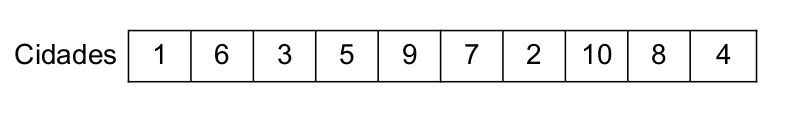
\includegraphics{arrayExample.png}}
	\caption{Exemplo de representação do problema.}
	\label{fig:arr}
\end{figure}

Um pré-processamento é realizado de modo que calculam-se as distâncias euclideanas entre todas as cidades e estes resultados são armazenados em uma tabela para consulta.

\subsection{Força Bruta}

A abordagem por força bruta considera todas as possíveis permutações entre as cidades, calculando a cada iteração o valor da rota presente; comparam-se então os valores para que se encontre o melhor (menor).

Levando-se em conta que nesta implementação é necessário considerar cada permutação entre as \textit{n} cidades de entrada, serão feitas comparações entre as \textit{n!} possíveis soluções e para cada permutação os n elementos são percorridos para somar as distâncias. Portanto, conclui-se que este algoritmo é da ordem \textit{O(n.n!)}.

\subsection{\textit{Backtracking}}

A solução por backtracking implementada foi uma adaptação de um algoritimo de permutações, porém a cada iteração o valor da distância é somado a uma variável usada para fazer a poda caso seja maior que a distância da rota mínima calculada até o momento. Como o algoritimo de backtracking tem a ordem de \textit{O(n.n!)}, esta é a ordem do nosso algoritimo no pior caso, porém com a poda o caso médio apresent melhora razoável.

\subsection{\textit{Simulated Annealing}}

O \textit{Simulated Annealing}, ou recozimento simulado, foi a meta-heurística utilizada na abordagem aproximada.

Proposto por Scoot Kirkpatrick, ele realiza o processo de busca por soluções ao simular o processo de recozimento de metais. Neste processo, o sólido é aquecido além de seu ponto de fusão e resfriado. Um resfriamento rápido conduz a produtos meta-estáveis, de maior energia interna, ao passo que um resfriamento lento conduz a produtos mais estáveis e de menor energia. Assim, o processo passa por vários estados possíveis ao longo do recozimento.

A analogia com um problema combinatório se dá pela Tabela \ref{fig:at}.

\begin{figure}[!ht]
	\centering
    \begin{tabular}{ | l | l | }
	    \hline 
        \textbf{Estados possíveis} & \textbf{Soluções} do espaço de busca
        \\\hline
        \textbf{Energia} & \textbf{Função objetivo}
        \\\hline
        \textbf{Energia mínima} & \textbf{Solução ótima} local, possivelmente local
        \\\hline
	\end{tabular}
	\caption{Analogia com problema combinatório.}
	\label{fig:at}
\end{figure}

A cada iteração, gera-se um novo estado a partir do estado corrente por uma pequena modificação aleatória; a troca de posição entre duas cidades, no caso presente. Caso esse novo estado apresente melhora em relação ao anterior, ele se torna o estado corrente. Em caso de piora, a probabilidade de se mudar do estado corrente para um novo estado é de $e^{-\Delta/(kT)}$, onde $\Delta$ é a diferença entre as soluções e \textit{kT} são constantes proporcionais ao processo de recozimento\cite{kirk}.

Em altas temperaturas, a chance de se aceitar um estado de piora é alta, de modo que cada solução possui praticamente a mesma probabilidade de ser a solução corrente. Ao longo do resfriamento, esta chance diminui, e a baixas temperaturas somente soluções com baixos valores terão alta probabilidade de se tornarem a solução corrente. 

Esta técnica permite que mínimos locais sejam evitados, o que garante uma solução melhor.

O comportamento do SA é descrito através de uma série de parâmetros variáveis. São eles:

\begin{itemize}
\item \textbf{Temperatura inicial ($T_0$)}: Representa a temperatura inicial, a qual deve ser alta o suficiente para permitir movimentos livres entre soluções vizinhas.
\item \textbf{Taxa de resfriamento ($\alpha$}): é a taxa de resfriamento, responsável pela velocidade na qual a temperatura resfria.
\item \textbf{SAmax}: número de interações a cada nível de temperatura.
\item \textbf{Tamanho do vetor (n)}: número de cidades envolvidas no problema.
\item \textbf{Temperatura final $T_f$}: uma temperatura mínima, próxima a zero, que indica a condição de parada.
\end{itemize}

O tempo de execução do algoritmo dependerá diretamente destes quatro parâmetros, uma vez que para uma temperatura inicial, haverá um decrescimento desta temperatura até a temperatura final; a velocidade deste decrescimento é determinada de modo que a cada iteração, a temperatura corrente é multiplicada pela taxa de resfriamento. Assim, este laço externo será executado $log_\alpha T_f/T$ vezes.

Para cada temperatura \textit{T} há SAmax iterações, dentro das quais calcula-se o valor da função objetivo (distância total percorrida) \textit{n} vezes.

Desta maneira, temos um algoritmo na ordem de O(pqn), onde p = $log_\alpha T_f/T$ e q = SAmax.


\newpage
\section{Resultados e Discussão}

Foram obtidos resultados apenas para o algoritimo \textit{Simulated Annealing}, não foi possivel obter resultados em tempo habil para os algoritimos de backtracking e força bruta. Os resultados obtidos foram:

\begin{table}[h]

\label{tab:cpu}
\centering
\begin{tabular}{| l | l | l | l |}
\hline
\textbf{Input} & \textbf{Alpha} & \textbf{Solução} & \textbf{Tempo} \\\hline
Berlin52 & 99 & 13620.6 & 749.9325 \\\hline
Berlin52 & 99 & 14404.7 & 885.378 \\\hline
Berlin52 & 90 & 23307.3 & 66.7996 \\\hline
Berlin52 & 90 & 26611.4 & 67.2125 \\\hline
Berlin52 & 85 & 23303.1 & 43.8778 \\\hline
Berlin52 & 85 & 26525.0 & 43.4335 \\\hline
Pr76     & 99 & 282312  & 802.966 \\\hline
Pr76     & 99 & 321372  & 803.845 \\\hline
Pr76     & 90 & 440157  & 77.211 \\\hline
Pr76     & 90 & 460295  & 76.9392 \\\hline
Pr76     & 85 & 470609  & 49.345 \\\hline
Pr76     & 85 & 497850  & 49.7831 \\\hline
Ch150    & 99 & 29289.8 & 1270.89 \\\hline
Ch150    & 99 &  &  \\\hline
Ch150    & 90 & 47363.3 & 108.695 \\\hline
Ch150    & 90 &  &  \\\hline
Ch150    & 85 & 48828   & 70.6719 \\\hline
Ch150    & 85 & 48609.6 & 70.3704 \\\hline
\end{tabular}
\caption{Resultados}
\end{table}
\newpage
Calculando as médias para cada variação dos algoritimos obtemos os resultados:

\begin{table}[h]
\label{tab:cpu}
\centering
\begin{tabular}{| l | l | l | l | l | l |}
\hline
\textbf{Input} & \textbf{Alpha} & \textbf{Solução} & \textbf{Referência} & \textbf{Sol. Exata} & \textbf{Tempo(s)} \\\hline
Berlin52 & 99 & 14,012.65 & 29948.3 & 7542   & 802.6553 \\\hline
Berlin52 & 90 & 24,959.35 & 29948.3 & 7542   & 67.0061  \\\hline
Berlin52 & 85 & 24,914.05 & 29948.3 & 7542   & 43.6557  \\\hline
Pr76     & 99 & 301,842   & 574570  & 108159 & 803.272  \\\hline
Pr76     & 90 & 450,226   & 574570  & 108159 & 77.075   \\\hline
Pr76     & 85 & 484,230   & 574570  & 108159 & 49.564   \\\hline
Ch150    & 99 &    & 53864   & 6528   & 803.406  \\\hline
Ch150    & 90 &    & 53864   & 6528   & 77.075   \\\hline
Ch150    & 85 & 48,718    & 53864   & 6528   & 70.521   \\\hline
\end{tabular}
\caption{ Média dos Resultados}
\end{table}

%inserir aqui comparações com a literatura

É possivel notar que quanto menor o valor de $\alpha$ menor o tempo de execução, porém mais longe do resultado otimo.

\newpage

\addcontentsline{toc}{section}{Bibliografia}
%\section*{Bibliografia}
\bibliography{bibliography}
\bibliographystyle{plain}
\newpage
\addcontentsline{toc}{section}{Anexo}
%\section*{Anexo}
\end{document}



